\section{Methodology}
\label{sec:methodology}

In our experience, teachers are not used to having access to tools
such as MiGen's TA tools, and their normal instinct is to walk
round the classroom in order to monitor how individual 
students are progressing and to help them.  
%Indeed, in the first two years of the MiGen project,
%before early versions of the TA tools were available, this was the
%strategy that teachers adopted in helping students who were
%undertaking learning tasks using the eXpresser.  
As discussed earlier,
this approach has significant limitations in an exploratory learning setting
due to the difficulty for the teacher 
to keep track of how a whole class of students are progressing, 
each at their individual pace and using their own
construction approach to the task at hand. Because of teachers'
general lack of experience with tools such as MiGen's TA tools, 
it was not possible for us to elicit from the outset a set of requirements 
for these tools from our teacher collaborators. Instead, it has been
necessary to adopt an iterative methodology comprising
successive phases of prototyping, requirements elicitation,
incremental development and evaluation, in collaboration with teachers. 

%\begin{figure}[htbp]
%  \centering
%  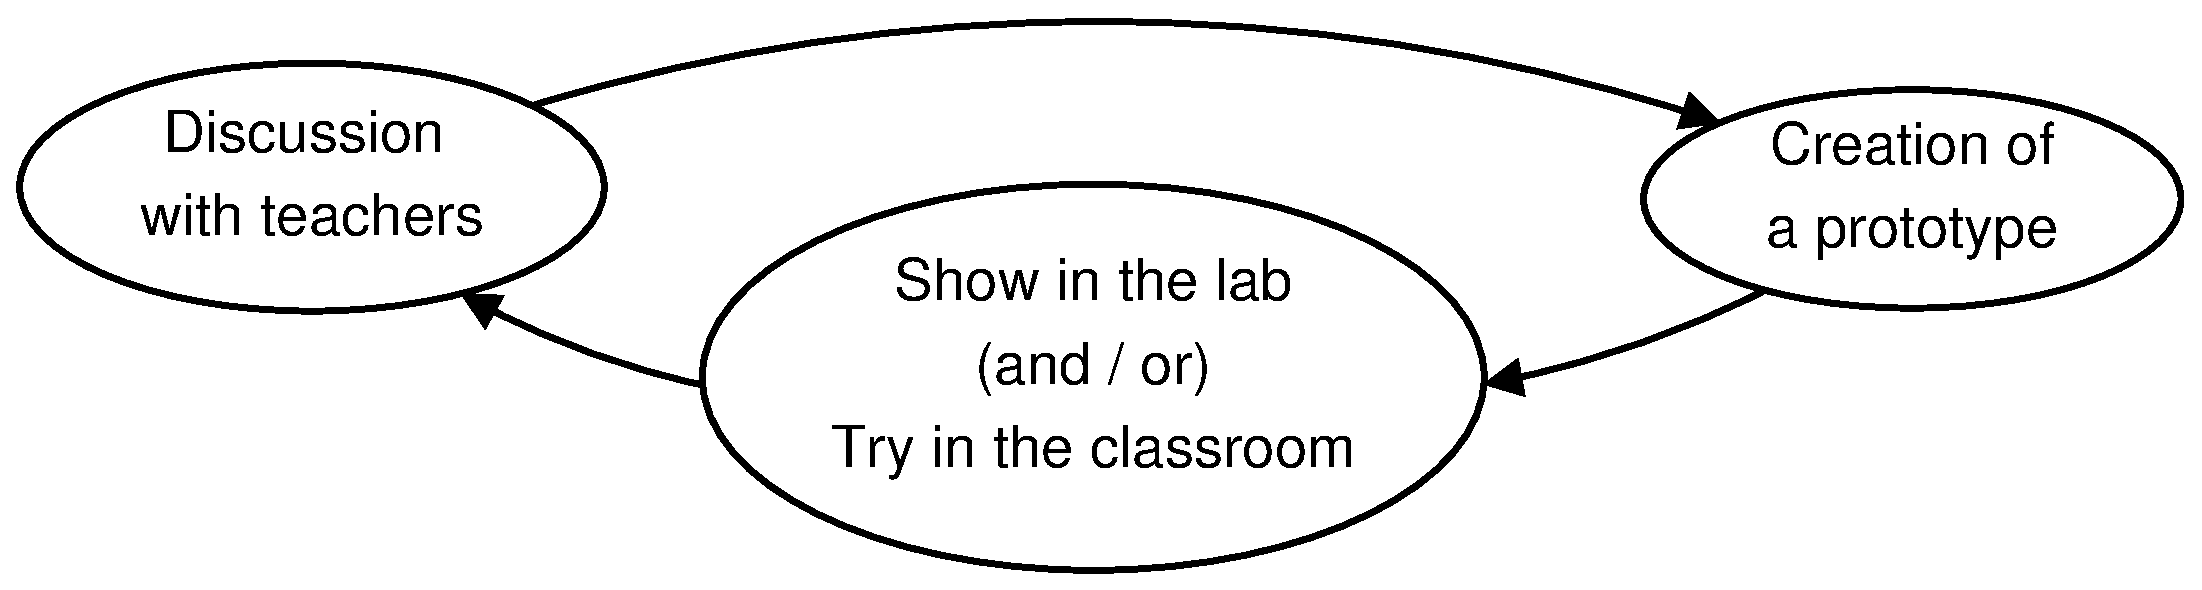
\includegraphics[width=\textwidth]{gfx/methodology.eps}
%  \caption{Iterative design with teachers}
%  \label{fig:it-teachers}
%\end{figure}

%In particular, the development of the TA tools has been undertaken in
%four phases during the course of the project, Phases A - D, which we
%describe below. The number of teachers with whom we have been able to
%collaborate closely during the course of the project is relatively
%small due to practical considerations of the available staff resources
%and the duration of the project. In particular,

Our Teacher Advisory group on the MiGen project comprised around 
20 maths teachers and mathematics educators
from a broad spectrum of secondary schools in the greater London area,
who attended regular project team meetings and gave their input to this 
process. However, the time that these teachers had
available to use early prototypes of the tools in their classrooms was
limited, and collaboration with a core group of 4 teachers
played a prominent role in this respect. 
 
\paragraph{Phase A}
\label{sec:phase}

After a first version of the eXpresser and of the student feedback
provided by the eGeneraliser had been developed during the first 15
months of the project, we undertook a first phase of prototyping and
requirements elicitation for the TA tools, working with our teacher
collaborators.    % January 2009 - June 2010
Mockups and
prototypes of several possible visualisations were developed and
discussed in meetings of the Teacher Advisory group and in one-to-one
interviews with those teachers who had trialled the eXpresser and
eGeneraliser in their classrooms. The aim of these interactions was to
elicit teachers' views about what information relating to students'
progress would be useful for them to have as
students are working on eXpresser tasks, and how they would like this
information to be presented.  
As an outcome of Phase~A, two visualisations were developed, 
which subsequently evolved into the Classroom Dynamics
(CD) and Student Tracking (ST) tool (see Section 4 below). 
Also identified were a preliminary set of TI and TD indicators
to be monitored by the system as students are working on the task
set and to be presented to the teacher by the ST tool.

\paragraph{Phase B}
\label{sec:phase-b}

The next phase of development of the TA tools began with several
classroom sessions trialling early prototypes of the ST tool with two teachers
in two schools. % July 2010 - December 2010 
These early trials are described in~\cite{IEEE-TLT-TA} and 
we refer the refer the reader to that paper for details. 
%
%Briefly, the first version of the ST tool was used in
%a classroom trial in July 2010. At that time, only event-based
%indicators were supported by the system, and one of the major items of
%feedback received from the teacher was that some of these indicators
%were actually showing changes in the {\em state} of the student rather
%than being single events, and should therefore be visualised as
%vertical bars in the display that change colour when their status
%changes. This feedback was incorporated into the development of the
%next version of the ST tool. Another major item of feedback from the
%teacher was that the set of indicators displayed by the ST tool should
%be expanded to show also when and what prompts are being generated by
%the system for each student. This feedback too was incorporated into
%the next version of the ST tool.
% 
%In September 2010, a second classroom trial of the eXpresser and ST
%tool was carried out with the same teacher using the new version of
%the ST tool, and also with another of our teacher collaborators in a
%different school. For both sessions, the ST tool was installed on the
%teacher's computer and we observed that the teachers afforded little
%time consulting the tool, spending most of their time in their
%familiar pattern of walking around the classroom to see what students
%were doing and to help them. 
%In post-lesson interviews, the two
%teachers suggested two ways of alleviating this problem: installing
%the Teacher tools on tablet PCs, which would then allow teachers to
%view these tools as they are walking around the classroom; and
%projecting the Teacher tools' display onto the whiteboard at the front
%of the class, again allowing teachers to monitor the progress of
%students as they are walking around the classroom. Both of these
%approaches were adopted for subsequent classroom trials of the system,
%in Phase D.
%
Following the classroom trials, one-to-one
interviews were held with the teachers so as to inform the further
development of the TA tools, and to gain insight into how the
teacher would use such tools in practice in the classroom. 
In these interviews, both teachers suggested that rather than
having the TA tools installed on the teacher's desktop PC, 
it would be preferable to install them
on a tablet PC; this would allow teachers to view the tools as they 
are walking around the classroom without having to keep returning back
to their desk. This approach was adopted 
for subsequent classroom trials of the tools in Phase D. 
% 
%Another major item of feedback received from both teachers was that
%the information being shown by the ST tool was too detailed to be useful to
%them during the lesson. However, they both felt it would be useful to
%be able to track this level of detail for individual students after
%the end of the lesson, for example for those students whose detailed
%progress they needed to check on before planning the next lesson. 
%%As a result of this feedback, we consulted in Phase C 
%%with the pedagogical experts on the project in deriving a subset 
%%of the most significant indicators to be displayed by default in the ST tool. 
%%Teachers can choose to `switch on' more indicators or `swich off' any of this
%%default set by means of an indicator-selection feature. 
%
The need for a third tool was also identified, 
which would show students' incremental achievement of the task goals during the lesson. 
This resulted in the development of the Goal Achievements (GA) tool (see Section 4).  
Finally, a set of Usage Scenarios for the whole suite of tools were identified, 
which we list as US1--US8 in Tables~\ref{tab:UsageScenariosA}
and~\ref{tab:UsageScenariosB}. 
These usage scenarios informed the development of the CD and GA tools,
and the design of the formative and summative evaluations of the 
whole suite of tools in Phases~C and~D. 

\begin{table}[htbp]
  \begin{tabular}{|p{0.5cm}|p{12.5cm}|}
  \hline \multirow{2}{*}{1} & \emph{Finding out which students need
    the teacher's
    immediate help.} \\
  \cline{2-2} & The teacher can consult the CD tool and see which
  students' circles are coloured Red. For any such student, the
  teacher can click on their circle to view their current model and
  rule, to provide some context for the help the teacher may then give
  the student. The teacher can also open up the ST tool to view the
  recent indicators relating to the students' actions, to provide
  additional context. If there are more than one student coloured Red
  in the CD display, the teacher may select to help first students who
  have achieved the fewest
  task goals. \\
  \hline \multirow{2}{*}{2} & \emph{Finding out which students are
    progressing satisfactorily towards completing the task and which
    students may be in difficulty} \\
  \cline{2-2} 
  & The teacher can consult the CD tool to see which
  students' circles are coloured Red. 
  If there is more than one student coloured Red,
  the teacher may select to help first the students who
  have achieved the fewest task goals. For any such student, the
  teacher can click on their circle to view their current model and
  rule, to provide some context for the help the teacher may then give
  to the student. The teacher can open up the ST tool to view the
  recent indicators relating to the students' actions, to provide
  additional context. The teacher can also up the GA tool to view specifically
  which task goals are being achieved by each student. 
  \\
  \hline \multirow{2}{*}{3} & \emph{Finding out which students are
    currently disengaged from the task.} \\
  \cline{2-2} 
  & The teacher can consult the CD tool and see which students'
  circles are currently coloured Amber. Looking at the number of goals
  each of these students has achieved, if a student has not completed
  the task goals, then she/he is likely to be currently disengaged
  from the task and in need of encouragement from the teacher. If a
  student has completed all the task goals, then she/he may need to be
  set additional goals or a new task to work on while waiting for the
  rest of the class to finish. \\
  \hline \multirow{2}{*}{4} & \emph{Identifying common conceptual and
    procedural difficulties students are facing in order to provide
    more explanation to the
    class as a whole.} \\
  \cline{2-2} 
  & Consulting the GA tool allows the teacher to see which
  task goals students are having difficulty completing, so as to
  inform additional explanation to the class.  Consulting the ST tool
  allows the teacher to see if there are specific Red indicators
  showing in many of the students' columns, indicating particular
  procedural difficulties that students may be facing and again
  informing the provision of additional explanation to the class.\\
  \hline
  \end{tabular}
  \caption{Usage Scenarios US1--US4}
  \label{tab:UsageScenariosA}
\end{table}
 
\begin{table}[htbp]
  \begin{tabular}{|p{0.5cm}|p{12.5cm}|}
  \hline \multirow{2}{*}{5}
  & \emph{Finding out which students have finished the task.} \\
  \cline{2-2}
  & The CD tool can be used to see which students have achieved all
  the task goals. For these students, the teacher can click on their
  circles to view their final model and rule, to check if they have
  achieved a correct solution. The teacher can then go to each student
  to set them a new task or additional goals relating to the current
  task, if their solution was correct; or ask them to reflect further
  on their construction if not. \\
  \hline \multirow{2}{*}{6}
  & \emph{Finding out which students have achieved which task goals.} \\
  \cline{2-2}
  & The GA tool can be used to see which students have achieved which
  of the task goals. \\
  \hline \multirow{2}{*}{7}
  & \emph{Providing appropriate support and guidance to individual
  students (i) during the lesson, and (ii) after the lesson.} \\
  \cline{2-2}
  &  This is a more open-ended use case which can be undertaken during
  the lesson using a combination of the tools as described for US1,
  US2, US3 above, and after the lesson by using the GA tool to see
  which task goals an individual student has not managed to achieve,
  the CD tool to view the student's final model and rule as produced
  by the end of the lesson, and the ST tool to view the student's
  detailed history of interactions
  during the lesson.  \\
  \hline \multirow{2}{*}{8}
  & \emph{Reflecting on the class' achievements and planning the next
  lesson.} \\
  \cline{2-2}
  &  Again, this is a more open-ended use case which can be undertaken by
  the teacher using a combination of the GA tool, to see which task
  goals have been largely achieved by the class, the CD tool to view
  selected students' models and rules, and the ST tool to see a
  historical record of how students tackled the task during the
  lesson.
   \\
  \hline
  \end{tabular}
  \caption{Usage Scenarios US5--US8}
  \label{tab:UsageScenariosB}
\end{table}
 
\paragraph{Phase C}
\label{sec:phase-c}

% Phase C 
% of development of the TA tools involved formative
% evaluation of the whole suite of tools with respect to the usage
% scenarios identified from Phase B (Phase C, January 2011 - May
% 2011). 
The formative evaluation was undertaken firstly with a group of trainee
maths teachers on a Postgraduate Certificate in Education programme
at the University of London, and subsequently with a group of pedagogical 
experts in maths education. We report on the design and outcomes of these formative
evaluation activities in Section 5.

\paragraph{Phase D}
\label{sec:phase-d}
 
The final phase of development of the TA tools % June 2011 - February 2012 
involved summative evaluation, undertaken in two parts. 
% In the first part, we conducted a classroom trial in which the
% teacher was first introduced to the TA tools before the lesson, and
% then used them during the lesson as students were working on a
% generalisation task in the eXpresser. 
% The teacher was asked questions
% by a member of the research team during and after the lesson, with the
% aim of evaluating the extent to which the TA tools meet the
% requirements of the usage scenarios. After having used the TA tools in
% one lesson, the same teacher was asked to undertake a similar lesson
% the next day, but this time without referring to the TA tools as she
% attempted to support the students working on a task in eXpresser. The
% aim of this second session was to compare the difference in the
% teacher's experience compared to the first lesson in which she could
% access the TA tools.
In the first part, we conducted two classroom trials, both with the same teacher
and the same class of students. In the first lesson, the teacher had access
to the TA tools to monitor students' progress and to support them 
as they were working on a task in eXpresser, whereas in the second lesson 
(held on the next day), the teacher was asked to conduct the lesson without 
referring to the TA tools. 
%
%The second part of the summative evaluation of Phase D involved a
%session held with a new cohort of trainee maths teachers on the
%Postgraduate Certificate in Education programme at the IoE. After
%introducing the eXpresser and TA tools to the participants and
%presenting common ways in which these could be used in the classroom,
%the participants were given access to the TA tools loaded with real
%data from the recent classroom sessions undertaken in the first part
%of the summative evaluation. They were given a questionnaire to probe
%their views about the usage and effectiveness of the TA tools as well
%as specific questions about the classroom status at specific times in
%the lesson, which they had to answer in a limited amount of time -
%simulating in this way the use of the tools in a real classroom.
The second part of the summative evaluation was undertaken with a 
new cohort of trainee maths teachers on the same Postgraduate 
Certificate in Education programme as in Phase C.  
We report on the design and outcomes of these summative evaluation
activities in Section 6.

 

%%% Local Variables:
%%% mode: latex
%%% TeX-master: "main"
%%% End:
